\centering
\small

\begin{tikzpicture}   % First subplot (low jitter) positioned relative to center
    \begin{axis}[
        at={(0,0)}, % Adjust position to the left, closer to the center
        anchor=center,
        width=\textwidth, height=.7\textwidth,
        xmin=20, xmax=80,
        ymin=-0.1, ymax=1.1,
        axis lines=none, % Remove axes
        title={low jitter}, % Add title
        title style={yshift=-10pt, color=muteblack}, % Adjust title position to make it closer to the plot
        ]
        % Plot individual waveforms (low jitter) in darkgray
        \addplot[darkgray,domain=20:80,samples=100] {exp(-0.5*((x-50)/5)^2)};
        \addplot[darkgray,domain=20:80,samples=100] {exp(-0.5*((x-52)/5)^2)};
        \addplot[darkgray,domain=20:80,samples=100] {exp(-0.5*((x-48)/5)^2)};
        \addplot[darkgray,domain=20:80,samples=100] {exp(-0.5*((x-51)/5)^2)};
        \addplot[darkgray,domain=20:80,samples=100] {exp(-0.5*((x-49)/5)^2)};

        % Plot average waveform (low jitter) in accent1 color, very thick
        \addplot[ultra thick,accent1,domain=20:80,samples=100] {exp(-0.5*((x-50)/5)^2)};
    \end{axis}
\end{tikzpicture}
\bigskip

\begin{tikzpicture}

   % Second subplot (high jitter) positioned relative to center
   \begin{axis}[
      at={(0.55\textwidth,0)}, % Adjust position to the left, closer to the center
       anchor=center,
        width=\textwidth, height=.7\textwidth,
       xmin=20, xmax=80,
       ymin=-0.1, ymax=1.1,
       axis lines=none, % Remove axes
       title={high jitter}, % Add title
       title style={yshift=-10pt, color=muteblack}, % Adjust title position to make it closer to the plot
       ]
       % Plot individual waveforms (high jitter) in darkgray
       \addplot[darkgray,domain=20:80,samples=100] {exp(-0.5*((x-45)/5)^2)};
       \addplot[darkgray,domain=20:80,samples=100] {exp(-0.5*((x-55)/5)^2)};
       \addplot[darkgray,domain=20:80,samples=100] {exp(-0.5*((x-40)/5)^2)};
       \addplot[darkgray,domain=20:80,samples=100] {exp(-0.5*((x-60)/5)^2)};
       \addplot[darkgray,domain=20:80,samples=100] {exp(-0.5*((x-50)/5)^2)};

       % Plot average waveform (high jitter) in accent1 color, very thick
       \addplot[ultra thick,accent1,domain=20:80,samples=100] {0.2*(exp(-0.5*((x-45)/5)^2) + exp(-0.5*((x-55)/5)^2) + exp(-0.5*((x-40)/5)^2) + exp(-0.5*((x-60)/5)^2) + exp(-0.5*((x-50)/5)^2))};
   \end{axis}
\end{tikzpicture}%
\bigskip

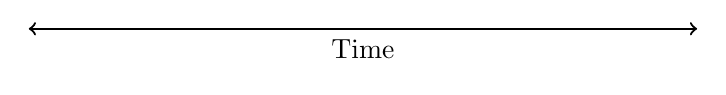
\begin{tikzpicture}
    % Draw the bottom horizontal axis
    \draw[thick,<->] (-0.35\textwidth,-1) -- (.35\textwidth,-1) node[pos=0.5,below] {Time};
\end{tikzpicture}
%\vspace{-5cm}
